\documentclass[13pt]{article}
%Gummi|065|=)
\title{\textbf{PRACTICA 6:AMPLIFICADORES OPERACIONALES.}}
\author{Guzman Vazquez Jaime Alan Yamil\\Rodriguez Lopez Francisco Javier.}
\date{31 de octubre}
\usepackage{graphicx}
\begin{document}

\maketitle

\section{PROCEDIMIENTO}
INVERSOR\\
Comenzaremos por explicar el amplificador operacional en su forma inversora en donde por medio de un voltaje de entrada y una resistencia en configuración lazo llamada RF, ademas de una resistencia a la entrada llamada Rin  por donde entrara el voltaje y la corriente, debido a que el amplificador operacional no permite la entrada de corriente, la corriente  escapa por el resistor en configuración lazo, debido a esto se puede decir que la corriente de entrada es igual a la corriente del resistor en la salida, la configuración inversora se determina la pata de entrada que se seleccione la resistencia de lazo ya sea positiva o negativa.\\\\
Para calcular la amplificación que entregara el circuito se debe hacer un calculo simple de amplificación dividiendo la resistencia de referencia, la que esta en la configuración del lazo de forma negativa (debido a su configuración inversora) entre la resistencia que esta en la entrada del amplificador operacional, esto daría el resultado de la amplificación que se espera para la onda de salida.\\\\

$$G=\frac{-RF}{Rin}$$\\
donde G es la ganacia del circuito.\\
RF es la resistencia en lazo.\\
Rin es la resistencia en la entrada del operacional.
\\\\Donde en el caso del circuito simulado da una ganacia de -10 veces.\\
El esquematico se muestra en el apartado de resultados.\\\\

NO INVERSOR.\\
En el caso de el amplificador operacional en configuración inversora es el mismo principio que en el inversor, los únicos cambios que se mostraran en en este seria que las entradas el voltaje de entrada sera direccionando a la pata positiva mientras que la resistencia en forma de lazo sera configurado en la pata negativa con anclaje a tierra.\\
ademas de esto en los cálculos el único cambio que se realizara es que la resistencia de referencia RF no esta de forma negativa esta vez puesto que es un amplificación no inversora y quedaría de esta forma:\\\\
$$G= \frac{RF}{Rin}$$\\
donde G es la ganancia del circuito.\\
RF es la resistencia en lazo.\\
Rin es la resistencia en la entrada del operacional.\\
\\En donde el circuito simulado da una ganancia de 10 veces el voltaje
SUMADOR\\
El funcionamiento del circuito sumador seria el agregar tensión a la salida del amplificador operacional para poder amplificar cualquier entrada de voltaje y entregar una salida mucho mas grande esto en función de la ganancia que puede entregar en función de las resistencias que se tienen.\\\\
Esta configuración sigue los mismo principios que la no inversora solo que este caso se agregan 5 resistencias mas debido a que el sumador que se realizo es de 3 entradas y cada una necesitaría 2 resistencias de entrada ademas de la resistencia de referencia común de todas como se muestra en el diagrama en el apartado de resultados.\\\\
El principal uso de este amplificador operacion en esta configuracion seria el de sumas 2 o mas voltajes para entregar un unico voltaje de salida es decir la suma de todos los voltajes de entrada, el calculo de este, para calcular el voltaje de salida seria simplemente dividir cada voltaje entre su resistencia y sumarlos para entregar el resistor Rin como se muestra a continuacion:\\\\
$$Vout=(\frac{V1}{R1}+\frac{V2}{R2}+\frac{V3}{R3}....)$$\\\\
donde Vout es el voltaje de salida.\\
V1 es la fuente numero uno (así sucesivamente con cada fuente.)
R1 sera la resistencia del voltaje 1 (así sucesivamente con cada resistencia.)\\\\En el circuito simulado dio un voltaje de salida de 400mV
 Asi sucesivamente hasta entregar la suma de todas las entradas de voltaje, si se tiene el mismo valor de resistencia se sumara unicamente entonces el voltaje  unicamente para saber cuanto voltaje saldrá.\\nota: se deben realizar igualmente los cálculos de ganancia anteriormente explicados.\\\\ 
RESTADOR\\
La configuración del tipo restador hace uso de una mezcla entre un amplificador inversor con uno no inversor, este resta una señal de la otra es decir la acción contraria que generaría el circuito sumador se aplica generalmente para eliminar el ruido que pueda contener una señal debido a cuestiones externas, esta configuración puede ser apreciada en el apartado de resultados en donde se muestra el diagrama del mismo ademas de la señal de salida que por supuesto entrega una señal menor de salida a la de entrada.\\\\
Los cálculos para esta serian los siguientes:\\\\ 

$$ Vout=V2(\frac{(R3+R1)R4}{(R4+R2)R1})-V1\frac{R3}{R1}$$\\
Donde Vout es el voltaje de salida\\
V2 seria el segundo voltaje.\\
V1 seria el primer voltaje .\\
R1,R2,R3... son las resistencias del circuito.\\ 
\\Los calculos de la simulacion dieron como resultado 100mv
DAC\\
Esta configuracion del amplificador operacional se utiliza para convertir señales digitales a señales analogas en donde se coloca una linea con un switch y una resistencia de por medio para evidenciar cada bit, si se queiren 4 bit se ponen 4 lineas como lo es en este caso posteriormente se pasa la señal al amplificador operacional en donde se forma el cambio de voltaje permitiendo que la señal que parece un representa un bit se de mostrado un incremento o decremento en la señal, al final teniendo una onda senoidal que es reconstruida con los picos mas altos del voltaje interpretandose como una señal analoga.\\\\
para que  se logre realizar esta tarea es necesario el generar el calculo para saber que valor debe tener la resistencia en funcion de el maximo voltaje que en el caso de la señal digital serian 5v formando el 1 logico mientras que el 0 logico es formado por los 0 voltios esto se realiza calculando seria el numero de voltios 5v para el 1 logico entre el numero de bit que se desean de la siguiente forma:\\\\
$$RIND=\frac{1logico}{bit deseados}$$\\
donde RIND representa el valor de cada resistencia en la linea.\\
1logico serian los 5v.\\
bit deseado los bit que seran necesarios en el circuito.\\
En el caso de la simulación dio 1.25 ohm en cada resistencia.\\\\

ADC\\
Este circuito toma la señal de 2 fuentes de voltaje y las compara en funcion de la otra enviando un 1 logico o un 0 logico dependiendo de la las fuentes y cual sea mayor la que esta conectada en la parte de el positivo de la entrada o la que esta en la entrada negativa de esta esto se va variando dependiendo de las resistencia que estan conectadas en serie que están divididas por solamente un switch estos para agrandar o aligerar la carga de ohms en el circuito permitiendo la comparación variable de los mismos, para esta configuracion de conversion se necesita de igual forma el calculo anterior para determinar la resistencia de cada circuito y en funcion de eso poner para que represente cada bit.\\
 
\section{RESULTADOS}
\begin{figure}[htp]
\centering
\includegraphics[scale=0.50]{/home/emile/Escritorio/guzman.vazquez.jaime.alan.yamil/practicas/EV_2_5_Arrelgos_de_amplificadores_de_potencia./imagenes simulaciones/INVERSOR.png}
\caption{Este es el diagrama que se siguió para el amplificador de potencia inversor.}
\label{.}

\end{figure}
\begin{figure}[htp]
\centering
\includegraphics[scale=0.20]{imagenes simulaciones/simulacion inversor.png}
\caption{}
\label{}
\end{figure}

\begin{figure}[htp]
\centering
\includegraphics[scale=0.50]{/home/emile/Escritorio/guzman.vazquez.jaime.alan.yamil/practicas/EV_2_5_Arrelgos_de_amplificadores_de_potencia./imagenes simulaciones/NO INVERSOR.png}
\caption{esquematico de amplificador no inversor.}
\label{.}
\end{figure}

\begin{figure}[htp]
\centering
\includegraphics[scale=0.20]{imagenes simulaciones/noinversosr.png}
\caption{}
\label{}
\end{figure}

\begin{figure}[htp]
\centering
\includegraphics[scale=0.50]{/home/emile/Escritorio/guzman.vazquez.jaime.alan.yamil/practicas/EV_2_5_Arrelgos_de_amplificadores_de_potencia./imagenes simulaciones/SUMADOR.png}
\caption{Esquematico de sumador de voltaje.}
\label{.}
\end{figure}

\begin{figure}[htp]
\centering
\includegraphics[scale=0.20]{imagenes simulaciones/sumador sim .png}
\caption{}
\label{}
\end{figure}

\begin{figure}[htp]
\centering
\includegraphics[scale=0.50]{/home/emile/Escritorio/guzman.vazquez.jaime.alan.yamil/practicas/EV_2_5_Arrelgos_de_amplificadores_de_potencia./imagenes simulaciones/RESTADOR.png}
\caption{Diagrama de restador de tension.}
\label{.}
\end{figure}

\begin{figure}[htp]
\centering
\includegraphics[scale=0.20]{imagenes simulaciones/restador sim .png}
\caption{}
\label{}
\end{figure}

\begin{figure}[htp]
\centering
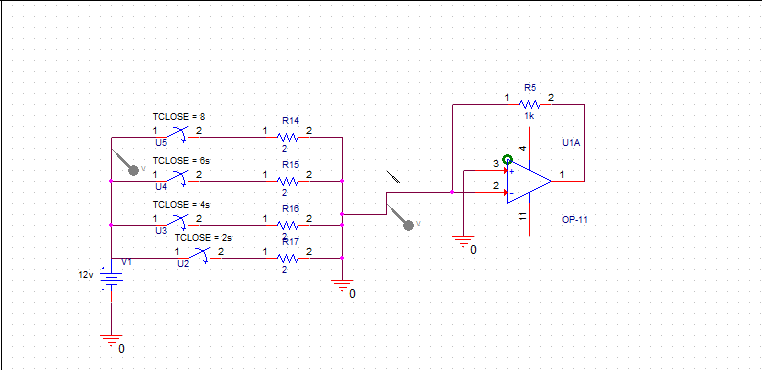
\includegraphics[scale=0.50]{/home/emile/Escritorio/guzman.vazquez.jaime.alan.yamil/practicas/EV_2_5_Arrelgos_de_amplificadores_de_potencia./imagenes simulaciones/DAC.png}
\caption{diagrama de convertidor digital a analogo.}
\label{.}
\end{figure}


\begin{figure}[htp]
\centering
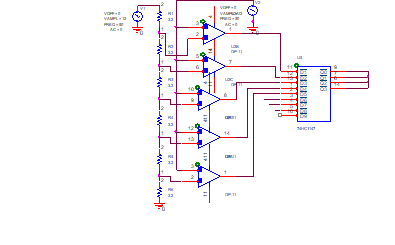
\includegraphics[scale=0.60]{/home/emile/Escritorio/guzman.vazquez.jaime.alan.yamil/practicas/EV_2_5_Arrelgos_de_amplificadores_de_potencia./imagenes simulaciones/ADC.png}
\caption{conversor Analogo a digital cambiar este puto.}
\label{.}
\end{figure}






















\section{CONCLUSIONES}
Jaime Guzman:\\
Las simulaciones que se realizaron son de gran importancia puesto que son todas en base a la utilización de amplificadores operacionales, ya sea el amplificar una señal, el restarle intesidad  a esta o el comparar dos entradas de voltaje para generar una respuesta y envia una señal son cuestiones que el amplificador operacional puede hacer, ademas de poder hacer muchas mas configuraciones.\\ estas aplicaciones son muy relevantes, ejemplificando esto tenemos las dos ultimas simulaciones que se realizan convertidores de señales analogicas a señales digitales y viceversa, esto es algo que practicamente se usa  en todo tipo de diferentes partes de la electronica, o de igual forma la amplificacion de señales es muy utilizada cuando las señales recividas son muy pequeñas o demasiado debiles, esto es de igual forma muy importante para cualquier ambito de la industria.  

\end{document}
